%%%%%%%%%%%%%%%%%%%%%%%%%%%%%%%%%%%%%%%%%%%%%%%%%%%%%%%%%%%%%%%%%%%%%%
% 平成12年度東京大学大学院理学系研究科物理学専攻修士課程入学試験
% 専攻 物理
% 問題5
%%%%%%%%%%%%%%%%%%%%%%%%%%%%%%%%%%%%%%%%%%%%%%%%%%%%%%%%%%%%%%%%%%%%%%
\documentclass[fleqn]{jbook}
\usepackage{physpub}

\begin{document}
\begin{question}{専攻 問題5}{吉川 真}
高速の荷電粒子が物質中を通過すると、物質の電離や励起が起きる。ある種の物質
 は、荷電粒子通過で生じた励起状態が基底状態に戻るときに可視光領域で発光す
 るので、それを利用して放射線検出に用いることが出来る。
\parbox{6.5cm}{
 \hspace*{1em}代表的な物質としてNaI結晶シンチレーターがある(Na及びIの質量
 数はそれぞれ
 23及び127、原子番号はそれぞれ11及び53、密度は、$3.7\Unit{g/cm^3}$である)。
 NaIシンチレーターと光電子増倍管を組み合わせて放射線検出を行う装置を模式的
 に示した右図を参考にして、以下の問いに答えよ。
 }
 \parbox{10cm}{
 \begin{center}
  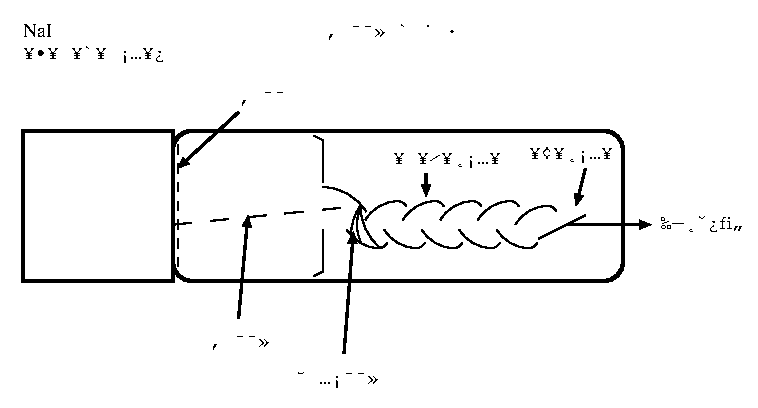
\includegraphics[width=9cm,keepaspectratio,clip]{1999phy5-1.eps}
 \end{center}
 }

\begin{subquestions}
 \SubQuestion 1kVの高電圧源が一台ある。これを用いて光電子増倍管を動作させ
 るには、各電極(光電面、ダイノード、アノード)にどのように電圧を供給すれば
 よいか、概略を示せ。また、アノードの出力を、放射線のエネルギーに比例した
 波高スペクトルとして記録するには、どのように信号処理をすればよいか、概略
 を示せ。

 \SubQuestion NaIの前面からNaIの中心に向けてエネルギー1MeVの単色電子線を入
 射し、波高スペクトルを記録したら、有限の巾を持ったピークが観測され、その
 ピーク巾(半値全巾)とピーク中心値の比率(分解能)は約5\%であった。分解能を決
 めている要因について論じよ。
 
 \SubQuestion 今度はNaIの前面からNaIの中心に向けてエネルギー1MeVの単色ガン
 マ線を入射し、波高スペクトルを記録した。NaIでガンマ線が測定できるのは何故
 か、簡潔に述べよ。また、どのような波高スペクトルが期待されるか、図で示し、
 説明を加えよ。

 \SubQuestion NaIの前面に薄い鉛板を張り、板の厚さを変えながら、板を通過し
 てNaIに入る放射線を測定した。線源の強さと測定時間は常に一定に保った。
 i)1MeVの電子が入射するとき、ii)1MeVのガンマ線入射するとき、の各々について、
 波高スペクトル(ピークの位置及び高さ等)が板の厚さとともにどう変化するか、
 概略を図示して説明せよ。

 \SubQuestion ある線源からのガンマ線スペクトルを測定しようとしたが線源の強
 度が極めて弱く、宇宙線μ粒子がバックグラウンドとして問題となることがわかっ
 た。測定系にどのような対策を施せば、このバックグラウンドを取り除くことが
 できるか具体的な方法を説明せよ。

 \SubQuestion 太陽からは、毎秒$1\Unit{cm^2}$あたり$7\Keta{10}$個の
 ニュートリノが降り注いでいる。ニュートリノがNaI結晶中の電子と相互作用を
 して、測定の邪
 魔になっていないか考えた。そのような相互作用は、1年間に何例ぐらい期
 待されるか計算式を示し、
 計算せよ。なお、NaI結晶の大きさは
 $5\Unit{cm}\times 5\Unit{cm}\times 5\Unit{cm}$の立方体とし、ニュート
 リノと電子との相互作用断面積は$1\Keta{-45}\Unit{cm^2}$、アボガドロ
 数は$6\Keta{23}$、一年は約$3\Keta{7}$秒とせよ。

\end{subquestions}
 
\end{question}
\begin{answer}{専攻 問題5}{吉川 真}
 \begin{subanswers}
  \SubAnswer
  (電圧供給)
  \begin{center}
   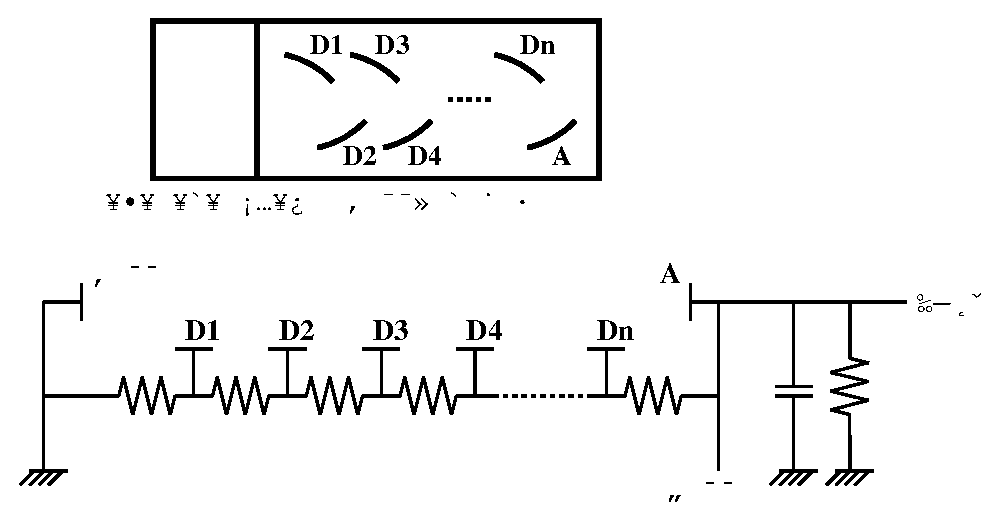
\includegraphics[width=10cm,clip]{1999phy5-2.eps}
  \end{center}
  上図の様に電位が徐々に上がっていくように回路を作ればよい。

  (アノード出力の信号処理)
  \begin{center}
    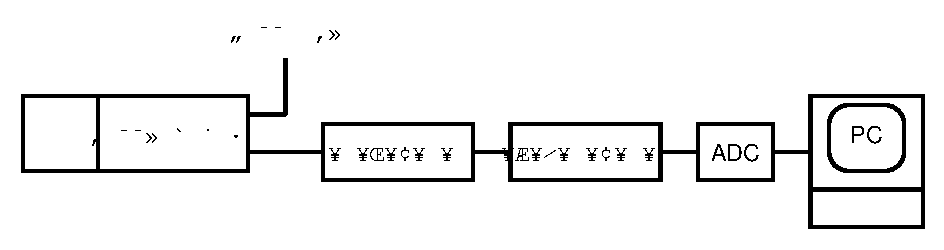
\includegraphics[width=12cm,clip]{1999phy5-3.eps}
  \end{center}
  アノードの出力のパルスをアンプで整形したのち、ADC(Analog to Digital
  Converter)でデジタル信号に変換しコンピュータに取り込む。

  \SubAnswer 分解能を決めている要因としては、初期の発光現象における発光光
  子数の統計的変動と、光電面から放出される有効光電子数の統計的変動が考えら
  れるが、NaI結晶シンチレータは発光量が非常に多いため、発光光子数の統計的
  変動は小さい。また、アンプなどの周辺機器からの電気的雑音も分解能を悪く
  する。

  \SubAnswer $\gamma$線は、物質との三種類の電磁相互作用(光電効果、コンプト
  ン散乱、電子対生成)により、電子を放出させる。その電子がシンチレータを励
  起することにより、$\gamma$線を測定することができる。
  \begin{center}
   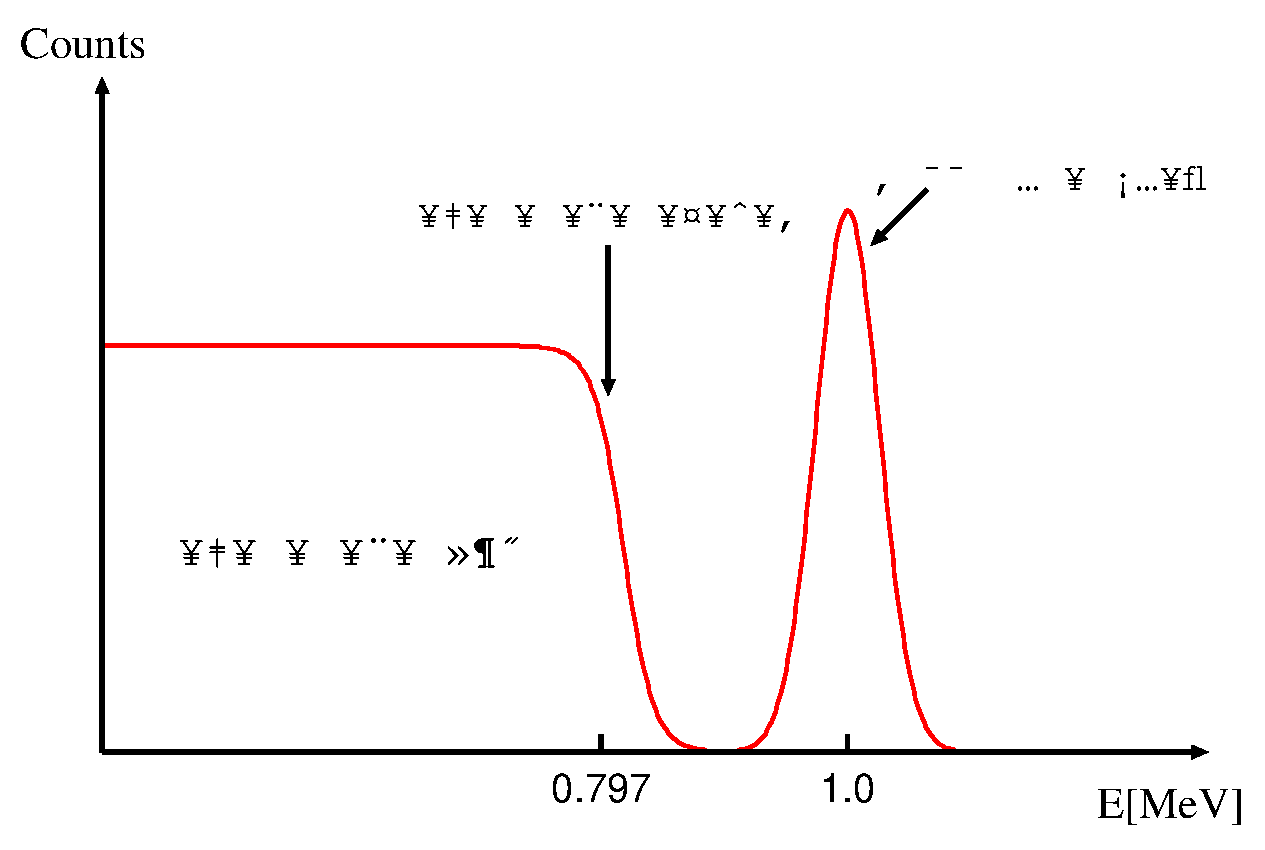
\includegraphics[width=8cm,clip]{1999phy5-4.eps}
  \end{center}

  上図の様な光電吸収ピークと、コンプトン散乱のスペクトルが得られる。コンプ
  トン散乱によるスペクトルは、散乱角$\theta$に依存するため、連続スペクトル
  となり、$\theta=180\deg$の時、最大となる。これがコンプトンエッジである。
  電子対生成は、$E_\gamma>2m_ec^2\quad(1.02\Unit{MeV})$の場合にのみ起こる
  ため、この場合は、電子対生成は起こらない。

  \SubAnswer
  \begin{subsubanswers}
   \SubSubAnswer $1\Unit{MeV}$の電子が入射するとき、
   \begin{center}
    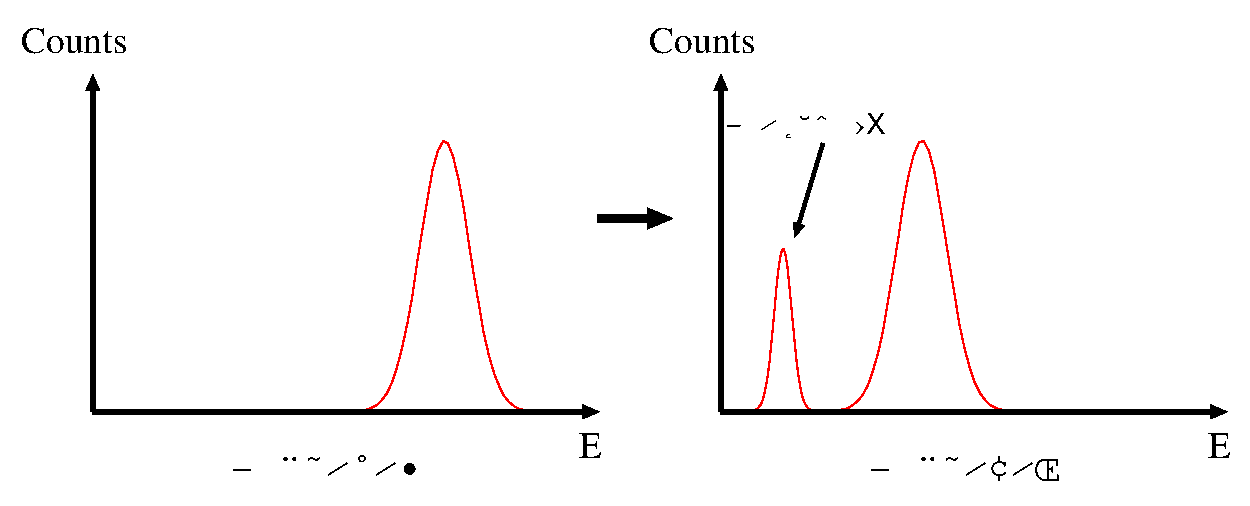
\includegraphics[width=12cm,clip]{1999phy5-5.eps}
   \end{center}
   
   電子は鉛板中の電子を散乱し、エネルギーを失うが、電子数は変化しない。従っ
   て、鉛板が厚くなるにつれて、ピークの位置が低エネルギー側へ移動するが、
   ピークの高さは変らない。

   \SubSubAnswer $1\Unit{MeV}$の$\gamma$線が入射するとき、
   \begin{center}
    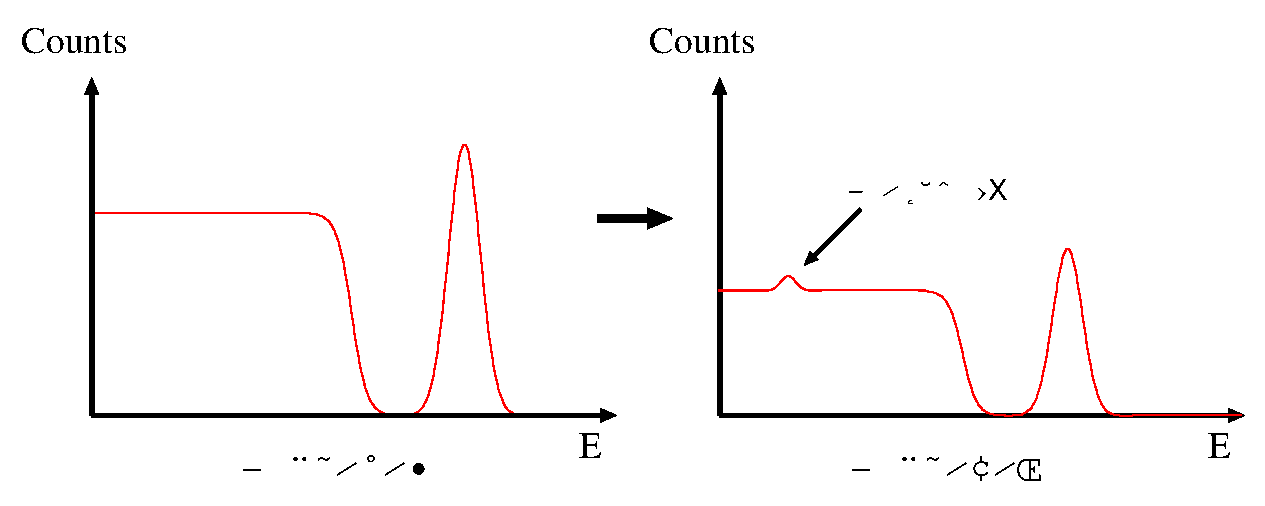
\includegraphics[width=12cm,clip]{1999phy5-6.eps}
   \end{center}

   鉛板が$\gamma$線を吸収するため、photon数が減少する。従って、ピークの位
   置は変化しないが、ピークの高さが低くなる。
  \end{subsubanswers} 

  \SubAnswer $\mu$粒子は物質との相互作用が弱いため、遮へいの効果は低い。従っ
  て、プラスチックシンチレータ等で主検出器全体を囲み、外部より入射してくる
  $\mu$粒子を検知して、主検出器の計数を除くという反同時計数を行なえばよい。

  \SubAnswer NaI結晶中の電子の総数は、
  \begin{eqnarray*}
   & (\mbox{密度})\times(\mbox{体積})\times(\mbox{1/分子量})
    \times(N_A)\times(\mbox{NaI一個当りの電子数}) & \\
   & 3.7\times5^3\times\frac{1}{150}\times(6\times10^{23})\times(53+11)
    & =1.2\times 10^{26}\mbox{個}
  \end{eqnarray*}
  従って、ニュートリノがNaI結晶中の電子と相互作用する数は、一年間で、
  \[
   (1.2\times10^{26})\times(1\times10^{-45})\times
  (7\times10^{10})\times(3\times10^7)=2.5\times10^{-1}\mbox{個}
  \]
  従って、一年間で、約$2.5\times10^{-1}$個検出される。
\end{subanswers}
\end{answer}


\end{document}
